\documentclass{acm_proc_article-sp}

%packages
\usepackage{epstopdf}
\usepackage{hyperref}
\usepackage{tikz}
\usepackage{algpseudocode}
\usepackage{algorithm}
\usepackage{cleveref}
\usepackage{todonotes}
\usepackage{cite}
\usepackage{pgfplots}
\usepackage{microtype}
\usepackage{siunitx}
\usepackage{tikz}
\usetikzlibrary{arrows,automata}
\usepackage{siunitx}
 
\DeclareSIUnit\Wh{Wh}

\begin{document}

\title{Fastest-Path Algorithm for Electrical Vehicles}

\numberofauthors{4} 
\author{
% 1st. author
		\alignauthor A. B. Eriksen\\
       \affaddr{Institute of Computer Science}\\
       \affaddr{Aalborg University}\\
       \email{aeriks11@student.aau.dk}
% 2nd. author
		\alignauthor M. A. Madsen\\
       \affaddr{Institute of Computer Science}\\
       \affaddr{Aalborg University}\\
       \email{mman10@student.aau.dk}
\and
% 3rd. author
		\alignauthor
		M. M. Andersen\\
       \affaddr{Institute of Computer Science}\\
       \affaddr{Aalborg University}\\
       \email{mama11@student.aau.dk}
% 4th. author
		\alignauthor
		S. B. Jensen\\
       \affaddr{Institute of Computer Science}\\
       \affaddr{Aalborg University}\\
       \email{sbje11@student.aau.dk}}
\date{30 July 2014}
\maketitle

\begin{abstract}
We describe a greedy-heuristic algorithm for finding the fastest path, between two points in a
large road network graph, for electrical vehicles. Unlike many of today's GPS systems, our greedy-heuristic 
algorithm takes both the drive time and the recharge time into account. Since the recharging possibilities for 
electrical vehicles are still limited on Danish roads and the recharging process takes a long time compared to 
refuelling times of regular gasoline cars, this is necessary in order to give the electrical vehicles users a 
useful route plan.\\

We compared the performance of the greedy-heuristic algorithm with a naive algorithm on road
networks extracted from OpenStreetMap (OSM). We modified the OSM road network, so it contained Danish speed limits
and charge stations. We compared the performance on four different parameters: the density of charge stations in
the road network, the quality of the charge stations in the road network, the size of the road network measured in 
distance and the complexity of the road network measured in number of nodes. The greedy-algorithm 
performed pretty god damn okay     

\end{abstract}

\keywords{Shortest-path algorithm with resource constraints, Electrical vehicles, Road-network, Route planing} % NOT required for Proceedings

\chapter{introduction}


\section{Electrical Vehicles}

We investigate the differences and similarities of two electric vehicles: the Nissan Leaf and Tesla's S model. 
One of the reasons why we have chosen these two cars in particular is the fact that both of the cars, today, 
are among the most popular electric vehicles. We investigate the range, charging options, charging times, 
battery capacity and other factors which may be relevant when calculating the fastest path between two points for 
electric vehicles.

\subsection{The Range}

The range of an electric vehicles depends on many factors, such as: the battery capacity, how efficient the battery
is used, the speed which is driven at, the drag of the car, the wind resistance, how much air conditioning is 
used etc. The two most important factors, though, are the battery capacity and the speed which is driven at. 
Tesla's S model comes with different battery sizes. We choose to focus on the Tesla S model with 85 kWh which is 
the biggest battery size but it also comes in a 60 kWh variant. The Nissan Leaf comes with a 24 kWh battery. The 
Nissan Leaf is said to have 120 km EPA rated range. EPA stands for Environmental Protection Agency 
\section{A Simpler Problem}

To make the problem of finding the fastest path between two points on a road network simpler, 
we assume the speed of the electric vehicle is constant and we assume the charging time at
charge stations is constant. 

\subsection{The graph representation}
We represent the road network as a graph where edges represents the roads and vertices represents
road intersections or charge stations. An edge is a double of time and cost:

\[E = (\textit{TIME}, \textit{COST}) \]

$\textit{TIME}$ represents the time it takes to pass an edge. $\textit{TIME}$ is the distance of
the road divided by the speed, but as mentioned earlier, for this simpler problem we assume
speed is constant, so $\textit{TIME}$ is given solely by the distance of the road. $\textit{COST}$ 
represents the energy cost for the an edge. $\textit{COST}$ is the energy usage per distance 
times the distance. Since the energy usage per distance is also given by the speed, this value
will be constant and so $\textit{COST}$ is solely given by the distance of the edge.

A vertex is a single of time: 
 
\[V = (\textit{TIME})\]

$\textit{TIME}$ is the time it takes to charge an electric vehicle one unit of energy e.g. minutes 
per kWh. The time it take to charge an electric vehicle one unit of energy depends on the current
capacity of the electric vehicle, but as mentioned earlier, for simplicity, we assume charging 
time is constant no matter the current capacity of the battery.

\subsection{A simple example}

We want to give a simple example of how an algorithm might work, for finding the fastest path 
between two points when the charging time is constant and the speed is constant. The example is
illustrated in \ref{fig:simpleexample}. We want to find the fastest path from $s$ to $t$. The
electric vehicle used has a battery capacity of 50 kWh. The unit of $\textit{TIME}$ for vertices
is minutes/kWh, the unit of $\textit{TIME}$ for edges is minutes and the unit of $\textit{COST}$
for edges is kWh. E.g. the edge (s, a) takes 10 minutes and costs 10 kWh to pass, and the charge
station at vertex a charges with a speed of 3 minutes/kWh. Vertices with the value $\infty$, are
considered intersections of roads and they are without charging stations.

   

\begin{figure}
\centering
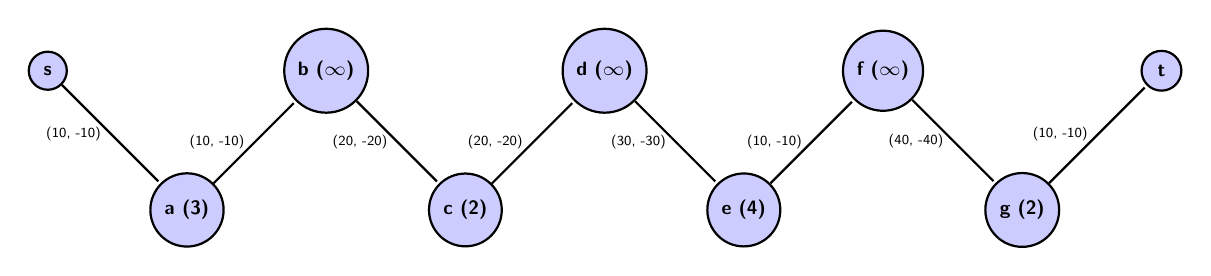
\begin{tikzpicture}
  [scale=.4,>=stealth',shorten >=1pt,auto,node distance=2.5cm,
  thick,main node/.style={circle,fill=blue!20,draw,font=\sffamily\scriptsize\bfseries}]
  \node[main node] (1) {s};
  \node[main node] (2) [below right of=1] {a (3)};
  \node[main node] (3) [above right of=2] {b ($\infty$)};
  \node[main node] (4) [below right of=3] {c (2)};
  \node[main node] (5) [above right of=4] {d ($\infty$)};
  \node[main node] (6) [below right of=5] {e (4)};
  \node[main node] (7) [above right of=6] {f ($\infty$)};
  \node[main node] (8) [below right of=7] {g (2)};
  \node[main node] (9) [above right of=8] {t};

  \path[every node/.style={font=\sffamily\tiny}] 
  (1) edge node [left] {(10, -10)} (2)
  (2) edge node [left] {(10, -10)} (3)
  (3) edge node [left] {(20, -20)} (4)
  (4) edge node [left] {(20, -20)} (5)
  (5) edge node [left] {(30, -30)} (6)
  (6) edge node [left] {(10, -10)} (7)
  (7) edge node [left] {(40, -40)} (8)
  (8) edge node [left] {(10, -10)} (9);
\end{tikzpicture}
\caption{Figure: Illustration of a simple road network with start point $s$ and end point $t$}
\label{fig:simpleexample}
\end{figure}

\section{The Optimisation problem}

We intend to find the fastest path between two points, s and t, for an electric vehicle. To find the fastest path we need to measure time. Time can be spend on two things: driving or charging. Since the charging times can vary a lot from charging station to charging station perhaps it would be fastest to take a slower path if it had a faster charging station on it. In more mathematical terms if we represent roads as vertices V and charging stations as edges E, if a charging station have a charging speed of 0 it is just an intersection. In plane test solving the problem of finding the fastest path in a graph is: 
minimizing the sum of time spend driving + the sum of time spend charging. 
\begin{equation}
\begin{aligned}
& \underset{x_{1 \dots n},y_{1 \dots n}}{\text{minimize}}
& & \sum_{j=1}^{n} \frac{C_j}{x_j} + \sum_{i=1}^{n} y_i \\
\end{aligned}
\end{equation}\label{eq:objfunction}
Where $x_j$ is the speed(km/h) of the EV driving when driving road segment $j$, $C_j$ is the distance(km) of road segment $j$, which means $\frac{C_j}{x_j}$ is time in hours. $y_i$ is the time spend at charging station $i$.  

For a solution to be feasible the following constrains need to be complied with: 
The most obvious constraint is the path constraint, the fastest path needs to be a path. 
\begin{gather}
e_1 = s \\
e_n = t \\
\forall{m \in 1 \dots n-1} \; (e_m, e_{m+1}) \in E 
\end{gather}\label{eq:pathconstraint} 
S and  t is the start and target node in the graph. E is the edges of the input graph.  
The feasibility of the solution is also bound by different physical factors, e.g. the amount of energy in the battery must be with the range of the battery's capacity and 0, further one can not charge for a negative time period. Lastly the electric vehicle need to drive within a specific speed range.     

\begin{gather}
\forall{m \in 1 \dots n} \; 0 \leq \sum_{i=1}^{m} \left( \int_{bat}^{y_i} e_i.f(z) \right) - \sum_{j=1}^{m} C_j*g(y_j) \leq batteryCapacity \\
\forall{j \in 1 \dots n} \; lb_j \leq x_j \leq up_j \\
\forall{i \in 1 \dots n} \; y_i \geq 0
\end{gather}\label{eq:physicalconstraints}
$e_i.f(z)$ is the charging function for the charge station located at edge i. $g(y_j)$ is the power consumption function. BatteryCapacity is the capacity of the EV's battery. 
$lb_j$ is the lower bound for the speed of the EV, $ub_j$ is the upper bound for the speed of the EV on road segment $j$. $bat$ is the amount of minutes the EV would have need to charge at the charging station it is currently at in order to have put the amount of kWh into the battery it has at arrival. When all of the above equations are combined we have the following optimization problem. 
\begin{equation}
\begin{aligned}
&\underset{x_{1 \dots n},y_{1 \dots n}}{\text{minimize}}
& &\sum_{j=1}^{n} \frac{C_j}{x_j} + \sum_{i=1}^{n} y_i \\
&subject to: \\
&&&e_1 = s \\
&&&e_n = t \\
&&&\forall{m \in 1 \dots n-1} \; (e_m, e_{m+1}) \in E \\
&&&\forall{m \in 1 \dots n} \; 0 \leq \sum_{i=1}^{m} \left( \int_{bat}^{y_i} e_i.f(z) \right) - \sum_{j=1}^{m} C_j*g(y_j) \leq batteryCapacity \\
&&&\forall{j \in 1 \dots n} \; lb_j \leq x_j \leq up_j \\
&&&\forall{i \in 1 \dots n} \; y_i \geq 0 
\end{aligned}
\end{equation} \label{eq:optiproblem}
The unknown parameters of the optimization problem is $x_{1\dots n}$ and $y_{1\dots n}$. 


\subsection{Techniques to help solving the problem}
To help solving the optimisation problem we think it would be interesting to further investigate the following techniques: branch and bound and Lagrange multipliers.
A branch-and-bound algorithm can be used to systematically enumerate  of all candidate solutions, where large subsets of candidates are discarded, by using upper and lower estimated bounds of the quantity being optimized. 
It is now yet clear if the problem can be modified so we can use Lagrange multipliers yet, in our current optimization problem equation \ref{eq:optipro} we are using constrained within ranges, where a problem being solved using Lagrange multipliers are subject to equality constraints.


%Min(Time(speed)) = Min(TimeSpendDriving(speed) + TimeSpendCharing(speed)) = Min



\section{Notation}
In this section we will briefly explain the mathematical notation and model used in the paper. The graph representation consists of edges which represents roads and vertices which represents either charge stations or road intersections. We define a \textbf{road network} as an ordered pair \(G=(V,E)\) comprising of a set $V$ of vertices together with a set $E$ of edges. Where $V$ is a finite set and $E$ is a binary relation on $V$. We further define the following functions:
\[ E_d(u,v)\rightarrow d \] 
\[ E_v(u,v)\rightarrow v \] 
These are partial functions defined by the edge $(u,v)$ and respectively returns a distance or a speed limit.

Each vertex is then defined as a \textit{charge station}, described by the following partial function:
\[V_c(v)\rightarrow c\]
A road intersection is simply a vertex with charge rate $c = 0$, while a charge station is a vertex where $c > 0$. An electrical vehicle is specified by two parameters: It's battery capacity ($kWh$), consumption rate ($kWh/km$). The consumption rate is given by the following function:

\[C_R(v)=av^2+bv+c\]
% \[ 4,60272*10^{-5}*v^2+6,59187*10^{-4}*v+0,173117 \] tesla

where $v$ is the speed of the vehicle. 

\begin{figure}
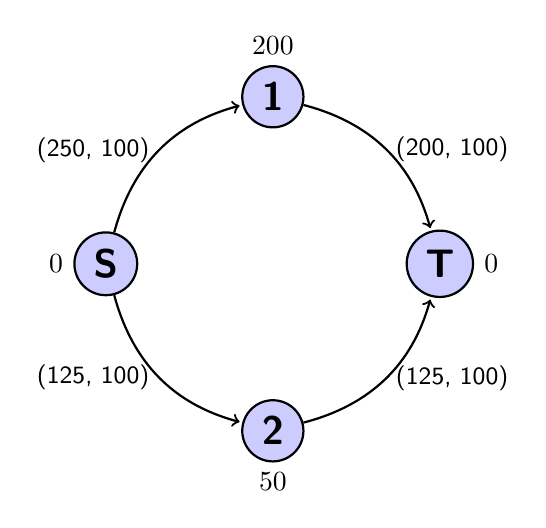
\begin{tikzpicture}[->,->,shorten >=1pt,auto,node distance=3cm,
  thick,main node/.style={circle,fill=blue!20,draw,font=\sffamily\Large\bfseries}]
%1
  \node[main node] (1) {1};
  \node[above] at (1.north) {200};
%2 
 \node[main node] (2) [below left of=1] {S};
  \node[left] at (2.west) {0};
%3 
 \node[main node] (3) [below right of=2] {2};
  \node[below] at (3.south) {50};
%4 
 \node[main node] (4) [below right of=1] {T};
  \node[right] at (4.east) {0};
%paths
  \path[every node/.style={font=\sffamily\small}]
    (1)
	  edge [bend left] node[right] {(200, 100)} (4)
    (2) edge [bend right] node[left] {(125, 100)} (3)
    	  edge [bend left] node[left] {(250, 100)} (1)
    (3) edge [bend right] node[right] {(125, 100)} (4)
    (4) ;
\end{tikzpicture}
\caption{A simple road-network with starting point $S$ and end point $T$}
\label{fig:simpleroad-network}
\end{figure}

\subsection{Problem Definition} % (fold)
\label{sub:problem_definition}
We are now ready to define the problem. The problem we are going to solve is defined as follows:
\begin{newdef}
Given a road network $RN=(V,E,D,v_{max},v_{min},R_{CH})$ and a vehicle $EV=(R_{CO},B_{cur},B_{cap})$. The fastest path from $s$ to $t$, is then defined as the path $P = \langle s,v_1,v_2,\dots,t \rangle$ where the time spent \emph{driving and charging} is minimal.
\end{newdef}



\subsection{Shorter does not imply faster}
\label{sec:shorternotfaster}
We will shortly investigate, which properties of paths are desirable. Firstly a shorter path does not necessarily imply a faster path for electric vehicles. This is partly due to the fact that electric vehicles use polynomially more energy as their speed increases, but also due to the fact that charge times on charging stations varies a lot. Driving a longer path with a fast charging station, can therefore turn out to be a faster choice than driving a shorter path with a slow charging station. This is illustrated in Figure \ref{fig:simpleroad-network}. In the example, we assume our car has a battery capacity of 100 $\si{\kWh}$ and a consumption rate of 0,4 $\si{\kWh\per\km}$ at the speed of 100 $\si{\km\per\hour}$.

Path 1 consists of two edges with distance: $ 250 \si{\km}$ and speed limit: $100 \si{\km\per\hour}$
and a charging station with a charge speed of 200 $\si{\kW}$. Path 2 consists of two edges with distance: $200 \si{\km}$ and speed limit: $100 \si{\km\hour}$ and a charging station with a charge speed of $30\si{\kW}$. The current battery capacity of the vehicle is noted at each vertex in parenthesis. The total time of each path:
				
\textbf{Path 1:} $\frac{250\si{km} + 250\si{km}}{100\si{\km\per\hour}} + \frac{100\si{\kWh}}{200\si{\kW}} = 5.5\si{\hour}$

\textbf{Path 2:} $\frac{200\si{km} + 200\si{km}}{100 \si{\km\per\hour}} + \frac{60\si{\kWh}}{30\si{\kW}} = 6\si{\hour}$


\begin{figure}
\centering
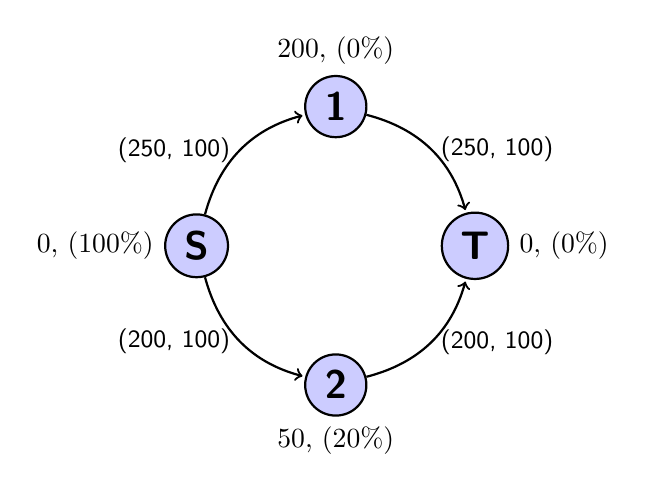
\begin{tikzpicture}[
->,->, shorten >=1pt,scale=0.1,node distance=2.5cm,thick,
main node/.style={circle,fill=blue!20,draw,font=\sffamily\Large\bfseries}]
%1
  \node[main node] (1) {1};
  \node[above] at (1.north) {200, (0\%)};
%2 
 \node[main node] (2) [below left of=1] {S};
  \node[left] at (2.west) {0, (100\%)};
%3 
 \node[main node] (3) [below right of=2] {2};
  \node[below] at (3.south) {50, (20\%)};
%4 
 \node[main node] (4) [below right of=1] {T};
  \node[right] at (4.east) {0, (0\%)};
%paths
  \path[every node/.style={font=\sffamily\small}]
    (1)
      edge [bend left] node[right] {(250, 100)} (4)
    (2) edge [bend right] node[left] {(200, 100)} (3)
          edge [bend left] node[left] {(250, 100)} (1)
    (3) edge [bend right] node[right] {(200, 100)} (4)
    (4) ;
\end{tikzpicture}
\label{fig:simpleroad-network}
\caption{A simple road network with starting point s and end point t. The charge rates on the road network dictates that the longer path is in fact the fastest}
\end{figure}

\section{Related Work}\label{sec:relatedwork}
To the best of our knowledge, there is no directly related research to the fastest path problem for electrical vehicles, which is the focus of this article. The fastest path problem is an instance of the constrained shortest path problem, which there are many applications of. There is a lot of work on the shortest path problem, mainly Dijkstra's algorithm \cite{dijkstra1959note} which is an interesting approach to the general shortest path problem.\\

Another relevant constrained shortest path problem, in the domain of electric vehicles, is working with energy-optimal routing, instead of the fastest path \cite{artmeier2010shortest}.\\

Lastly, many commercial navigation services, introduce hierarchical substructures to perform the shortest path computation faster. This is known as contraction hierarchies, it is a concept which could also be applied to the approach introduced in this article, it is however not the main concern of research. It is mostly a speed-up technique for shortest path computation.




possible subjects
\begin{itemize}
    \item shortest path (dijkstra)
    \item 
\end{itemize}


% \section{Fastest Path}

Finding the fastest path for an EV, from vertex $s$ to $t$ in a road network, does not only depend on the lengths and speed limits of the road network's edges but also on the charge rates of it's vertices. We showed this in \Cref{sec:shorternotfaster}. This problem issues that a different approach needs to be taken, in order to solve a path fastest possible. In this section, we present a greedy heuristic algorithm for solving the fastest path problem.  

\section{Greedy Heuristic Algorithm}

\begin{frame}{Example}
    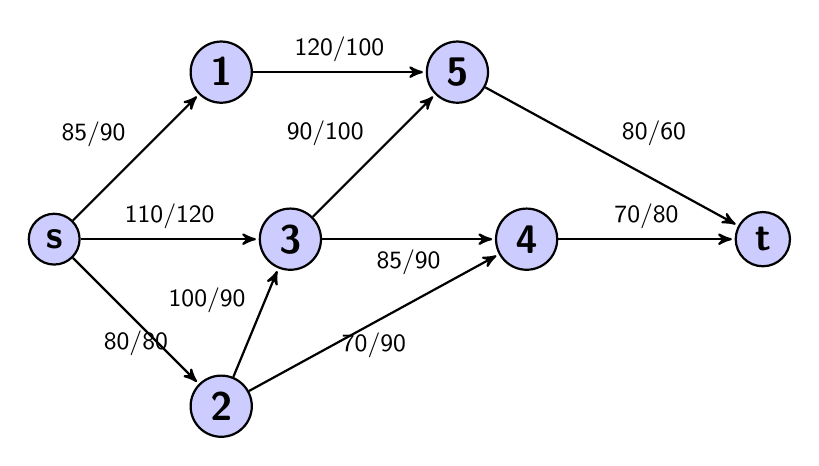
\begin{tikzpicture}[->,>=stealth',shorten >=1pt,auto,node distance=3cm,
  thick,main node/.style={circle,fill=blue!20,draw,font=\sffamily\Large\bfseries}]

  \node[main node] (s) {s};
  \node[main node] (1) [above right of=s] {1};
  \node[main node] (2) [below right of=s] {2};
  \node[main node] (3) [right of=s] {3};
  \node[main node] (4) [right of=3] {4};
  \node[main node] (5) [right of=1] {5};
  \node[main node] (t) [right of=4] {t};


  \path[every node/.style={font=\sffamily\small}]
      (s) edge node {85/90} (1)
      (s) edge node [below] {80/80} (2)
      (s) edge node {110/120} (3)

      (1) edge node {120/100} (5)

      (2) edge node {100/90} (3)
      (2) edge node [below] {70/90} (4)

      (3) edge node [below] {85/90} (4)
      (3) edge node {90/100} (5)

      (4) edge node {70/80} (t)

      (5) edge node {80/60} (t);
\end{tikzpicture}

\end{frame}


\subsection{Global optimal solution}
In this section an approach to finding a global optimal solution to the optimisation problem proposed in Section \ref{sec:optiprob}. The optimisation problem is a non-linear optimisation problem, due to $\frac{D(e_i)}{v_{e_i}}$ and $R_{CO}(v_{e_i})$ being non-linear function. The problem can however be reformulated into a linear programming problem by reformulating $\frac{D(e_i)}{v_{e_i}}$ and $R_{CO}(v_{e_i})$ as a piecewise-linear functions. Precisely the problem is modelled as a MIP problem. This section introduces the constraints necessary to solve the problem as a MIP problem and thereby end up at a global optimal solution.
\todo[inline]{Missing some references, and an explanation of what MIP is}

\subsubsection{Linearisation}
To handle the linearisation we need to introduce three new sets, a set of known variables which is the function of each linear piece, and another set of known variables which is the starting point of each line segment and a set of unknown variables which will be the line segments which produces the best result. The unknown variable is called SL(selected line) and it is two dimensional the first dimension is the the number of function to be solved and the second is the amount of pieces the function is split into. This lead to the following constraints.   
Exactly one line segment needs to be selected for all line segments. 
\begin{equation*}
\forall_{i\in1 \dots n }:\; \sum_{j=1}^{m} SL_{i,j} = 1
\end{equation*}
$n$ is the length of the path, $m$ is the amount of lines a line is split into and $\sum_{j=1}^{m} SL_{i,j} = 1$ ensures that only one line segments can be selected. 
Being that exactly one line segment needs to be chosen so SL needs to be binary values. 
\begin{equation*}
\forall_{i\in1 \dots n, j \in 1 \dots m}: \; \; SL_{i,j} \in{0,1} 
\end{equation*}
The speed of the EV needs to be constraint by the line segment chosen
\begin{equation*}
\forall_{i\in1 \dots n, j \in 1 \dots m-1}:\; SL_{i,j} * P_{i,j}  \le  v_{j,e_i} \le SL_{i,j}*P_{i,j+1}
\end{equation*}
$P$ is a set of start points of all line segments including the end point of the last segment. $SL_{i,j} * P_{i,j}$ is the minimal speed the EV is allowed to drive on edge $i$ and $SL_{i,j}*P_{i,j+1}$ is the maximal speed, note that the values will either be a valid value or $0$ if the segment is not selected. $P_{i,j+1}$ is the end point of $P_{i,j}$. 
The optimal solution to $\frac{D(e_i)}{v_{e_i}}$ or $R_{CO}(v_{e_i})$ can now be found by multiplying the slope of the selected line with the selected speed and adding the constant b. As an example the way to model $R_{CO}(v_{e_i})$ for $i$
\begin{equation*}
\sum_{j=1}^{m} LinesA_{i,j}*v_{j,e_i} + \sum_{j=1}^{m} SL_{i,j}*LinesB_{i,j} 
\end{equation*}
$\sum_{j=1}^{m} LinesA_{i,j}*v_{j,e_i}$ is equlent of $a*x$ and $\sum_{j=1}^{m} SL_{i,j}*LinesB_{i,j}$ is equlent of $b$. 
Finally note that this is a way to determine the solution of $\frac{D(e_i)}{v_{e_i}}$ or $R_{CO}(v_{e_i})$ and before the solution can be found the line segments and points for each of both of the non linear functions needs to be precomputed. 

%sources
%1, SWP-3587
%2, glpk-sos2




\section{Experiments}
\label{sec:experiments}
Now we present the experiments of the Greedy Heuristic Algorithm. It was concluded that the practical usage of the linear programming solution was not plausible in our experiments, after several implementations using an existing solver. Additionally, there will be a runtime complexity test of the algorithms.

We have constructed four experiments, to figure out what implication the adjusting of these parameters will have on the Greedy Heuristic Algorithm. The four parameters being experimented on are:
\begin{itemize}
     \item Route driving distance
     \item Charge rate of charge stations
     \item Consumption rate of EVs
     \item Density of charge stations
 \end{itemize} 

\todo[inline]{insert default values}


\subsection{Road network dataset} 
\label{sub:setup}
To facilitate the experiments, we've had to find a real world road network dataset which contains road distances, speed limits and charge stations of varying charge rates. Such a dataset does not openly exist to our knowledge. Instead we have used OpenStreetMaps which is an open-source collection of map data. One can read more about OSM at \url{http://www.openstreetmap.org/about}. OSM has a concept of ways and nodes. Ways represent geographical planar objects e.g. roads, cycleways, foot ways etc. A Node is a geographical point consisting of a latitude and longitude coordinate. A way is constituted of a set of nodes and some tags which describe meta-information about the way, such as the name of the way and what type of way it is e.g. a road, cycleway, foot way  etc. From this information we can derive that if way $e_1$ and $e_2$ intersect in node $u$, they will share the node $u$, which is what we refer to as an intersection/charge station in the road network.\\

The ways and nodes can easily be converted into a, for us, useful road network structure for experimenting. This is done, by simply filtering away all types of ways accept roads and use these as edges for our road network. To get a notion of speed limits on edges, we can derive general speed limits from the type of the roads. OSM carries such information as whether the road is a motorway, residential way, tertiary way etc. The speed limits are set according to Danish speed limits. For nodes, we are only interested in the ones which correspond to intersections between two roads. All other nodes in the road network are ignored. To get a notion of charge rate on the nodes we have implemented a method which distributes random charge rates on randomly selected nodes in the road network.

We have used the drivable part of Denmark as a baseline for the experiments. The dataset features:
\begin{itemize}
    \item 483407 vertices
    \item 543482 edges
\end{itemize}

\subsection{Naive algorithm}
\label{sub:naivealgorithm}
We have formulated a naive algorithm for performance comparison with our greedy-heuristic algorithm. The naive algorithm should simulate the way an naive electric vehicle driver would choose to travel through a road network. The naive algorithm works the following way: It greedily chooses the fastest roads in terms of distance over speed. Whenever the battery reaches 10 \% battery capacity, it starts searching for nearby charge stations in the radius allowed by the 10 \% battery capacity given the vehicles consumption rate. If no charge stations are available, the naive algorithm will go back to the time where it had 20 \% battery capacity and perform a search again. If still no charge stations are available, it will backtrack to the time where the vehicle had 30 \% battery capacity and so on. If no charge stations are available even with 100 \% battery capacity, the path from s to t is not possible. If, on the other hand, one or more charge stations are reachable, the algorithm will choose the closest one and charge to 100 \% battery capacity and resume greedily choosing the fastest roads from the charge station to t, in terms of distance over speed.

\subsection{Experiment: Complexity of Road Network}

We compared the run-time of the Greedy-heuristic algorithm to the naive algorithm with the complexity of the road network as changing parameter. The
complexity is measured in the number of nodes on the road network. The more nodes on the road network, the more nodes the two algorithms has 
to visit before they are able to find a fastest path. The set-up of the experiment: distance to drive was 100 km, the minimum distance between 
charge stations was 20 km. The initial number of nodes in the road network: 450000 nodes. The number of nodes is then counted down with 10000 nodes 
for each iteration of the test. The resulting graph is illustrated in (REF!).

\subsection{Experiment: Density of Charge Stations}

We compared the performance of the Greedy-heuristic algorithm to the naive algorithm with the density of charge stations as changing parameter. The
density of charge stations are measured in the minimum distance between two charge stations. Initially, the minimum distance is set to 5 km which generates 3029 charge stations in Denmark. Table \ref{table:chargedensity} shows the number of charge stations according to the minimum distance between charge stations in the road network.

\begin{table}[!htb]
\centering
		\begin{tabular}{ p{1.85cm} p{0.67cm} p{0.63cm} p{0.63cm} p{0.63cm} p{0.63cm} p{0.63cm} } \hline
		Radius (km): & 5 & 10 & 20 & 30 & 40 & 50 \\ \hline
		Stations: & 3029 & 827 & 326 & 117 & 76 & 49 \\ \hline 
		\end{tabular}
		\caption{number of charge stations corresponding to the minimum distance between two charge stations}
	\label{table:chargedensity}
	\end{table}

The set-up of the experiment: the distance to drive was set to 200 km, the complexity of the road network was 483398 nodes, which is the number of nodes in Denmark. The charge rates of the charge stations are evenly distributed with rates between $10 \si{\kW}$ and $100 \si{\kW}$. The resulting graph is illustrated in (REF!).

\subsection{Experiment: Charge Rate on Charge Stations}

We compared the performance of the Greedy-heuristic algorithm to the naive algorithm with the charge rate of charge stations as changing parameter. The minimum distance between charge stations was set to 30 km, the distance to drive was set to 200 km. The initial charge rates in the road network were evenly distributed between $10 \si{\kW}$ and $100 \si{\kW}$. For each iteration all charge rates are scaled with a constant factor resulting in worse of better charge rates on all charge stations. The resulting graph of the experiment is seen in (REF!). On the x-axis is displayed the average charge rate of the charge stations on the road network. On the y-axis is displayed the time it takes to pass a path of length 200 km. 

\subsection{Experiment: Size of Road Network}



\input{content/citations}

\section{Conclusions}
As the adoption rate of EVs increases time-optimised route planning systems for electrical vehicles will become increasingly important. 
We showed that a route planning system for EVs should be different from a system for traditional gasoline vehicles, since the time spend 
charging an EV is significantly longer than the time spend fuelling a gasoline vehicle. 

The problem of finding a route plan for an EV can be modelled as an optimisation problem, which can be solved by e.g. a linear programming system. We implemented a linear programming solution using GNU Linear Programming Kit and found that solving every simple path in a graph with the size of a real world road network, is simply too expensive to compute within reasonable time. Instead we presented a greedy heuristic algorithm that uses greedy choices and heuristics about the EV and the road network.

To benchmark the greedy heuristic algorithm we ran several experiments on a real world road network and compared the performance with a naive algorithm that simulated the pattern of a naive electric vehicle driver. The experiments showed that the greedy heuristic algorithm both finds better paths and better charging plans in the road network. The running time is however significantly larger than the naive algorithm.

We further compared the path time outputted by the greedy heuristic algorithm to the path time of the linear programming solution when run on the same path.
  

%ACKNOWLEDGMENTS are optional
%\input{content/acknowledgement}

\subsection{References}
\bibliography{tex}
\bibliographystyle{plain}

\end{document}
